% Generated by scripts/generate_int4_latex.py from the reviewed Markdown.
% Edit the Markdown source, then regenerate this file to keep both artifacts aligned.
\documentclass[10pt]{article}

\usepackage[letterpaper,textwidth=6.25in,textheight=9in]{geometry}
\usepackage{newtxtext,newtxmath}
\usepackage{amsmath}
\usepackage{array,booktabs,calc,longtable}
\usepackage{graphicx}
\usepackage{float}
\usepackage{microtype}
\usepackage{enumitem}
\usepackage{caption}
\usepackage{float}
\usepackage[numbers,sort&compress]{natbib}
\usepackage{titlesec}
\usepackage{hyperref}
\usepackage{xcolor}
\usepackage{etoolbox}

\definecolor{linkblue}{HTML}{245C8A}
\hypersetup{
  colorlinks=true,
  linkcolor=linkblue,
  citecolor=linkblue,
  urlcolor=linkblue,
  pdftitle={Value Differencing Halves 4-Bit Quantization Damage in Attention},
  pdfauthor={David Gao}
}

\setlist{nosep,leftmargin=1.35em}
\setlength{\parindent}{1em}
\setlength{\parskip}{0.12em}
\setlength{\tabcolsep}{4pt}
\setlength{\LTleft}{0pt}
\setlength{\LTright}{0pt}
\AtBeginEnvironment{longtable}{\footnotesize}
\captionsetup{font=small,labelfont=bf}
\emergencystretch=3em
\titleformat{\section}{\large\bfseries}{\thesection}{0.7em}{}
\titleformat{\subsection}{\normalsize\bfseries}{\thesubsection}{0.65em}{}
\titlespacing*{\section}{0pt}{1.35em}{0.55em}
\titlespacing*{\subsection}{0pt}{1.0em}{0.35em}

\providecommand{\tightlist}{\setlength{\itemsep}{0pt}\setlength{\parskip}{0pt}}
\providecommand{\pandocbounded}[1]{#1}
\newcounter{none}
\makeatletter
\def\maxwidth{\ifdim\Gin@nat@width>\linewidth\linewidth\else\Gin@nat@width\fi}
\def\maxheight{\ifdim\Gin@nat@height>0.72\textheight 0.72\textheight\else\Gin@nat@height\fi}
\makeatother
\setkeys{Gin}{width=\maxwidth,height=\maxheight,keepaspectratio}

\title{\textbf{Value Differencing Halves 4-Bit Quantization Damage in Attention}}
\author{David Gao}
\date{July 2026}

\begin{document}
\maketitle

\begin{abstract}
I began with a representational question: if neighboring token values become redundant with depth, should deep attention transmit what changed rather than repeat the raw value? I tested a one-line modification that subtracts the previous token's value projection with a coefficient that increases from zero to one across layers. It did not improve full-precision language modeling. At 20,000 matched training steps, the modified 27M-parameter models finished 0.0025--0.0066 BPB behind standard attention. The unexpected result appeared after weights-only 4-bit quantization: value differencing reduced W4 damage by 18.9\% and 22.3\% in two seeds, leaving the quantized models 0.0098 and 0.0178 BPB ahead. I then traced the effect to the architecture itself. Quantizing only attention weights cut damage by about half, and the value projection accounted for roughly 81\% of that gap in both seeds. RMSE-matched Gaussian perturbations of attention weights produced the same ordering in all six paired controls, showing that the result is not specific to round-to-nearest quantization. The current implementation trains 6.7\% slower and does not win at matched wall clock, so I claim a small-scale result about lower local sensitivity of attention parameters, not a production-efficiency result.
\end{abstract}

\bibliographystyle{plainnat}

\section{Introduction}\label{introduction}

Architecture studies usually stop at full precision. Deployment does not. Weights may later be rounded to four bits, pruned, or transformed by a calibrated quantizer, and two models that look equivalent before that step need not remain equivalent afterward.

This paper began somewhere else. I was studying adjacent-token redundancy in the values carried by attention. The measurements suggested a simple idea: deeper layers might transmit local changes more effectively than repeated raw content. I encoded that idea as \emph{depth-scheduled value differencing}.\footnote{Earlier project artifacts use the name ``DG Attention.'\,' I use the descriptive term \emph{value differencing} in this paper.} Early layers use ordinary values; each deeper layer subtracts more of the preceding token's value projection; the final layer transmits the full difference.

The full-precision result was unremarkable. Across the two final 20K runs, value differencing was slightly worse than standard attention. The interesting result emerged only after I rounded the large attention and MLP weight matrices to signed 4-bit values. That operation reversed the model ordering in both seeds: the modified checkpoints lost less quality and finished better after quantization.

That reversal could have been a measurement artifact or a property of some unrelated module. I therefore treated it as a question, not a conclusion. A component-by-component evaluation localized the gap to attention weights and, more specifically, to the value projection changed by the architecture. Quantization error itself was nearly unchanged, yet its effect on validation loss was roughly halved. Random attention-weight perturbations matched to the same relative RMSE produced the same result. Together, these controls support a precise conclusion: in this setting, training with value differencing makes the model less sensitive to perturbations of its attention parameters.

The scope is deliberately narrow. I study two training seeds, 27M-parameter FineWeb models, one tokenizer, one MLP family, BPB, and a calibration-free per-row W4 baseline. I do not claim a faster model, a production quantizer, or generalization to larger scales. The contribution is the localized empirical result and the sequence of controls that reduced a broad architectural idea to something the evidence actually supports.

\section{Value Differencing}\label{value-differencing}

\subsection{Architecture}\label{architecture}

Let \(x_{\ell,t}\) be the hidden state at layer \(\ell\) and token position \(t\). Standard attention projects it into queries, keys, and values. I leave the query and key paths unchanged and replace only the value payload:

\[
p_{\ell,t}=W^{(\ell)}_Vx_{\ell,t}, \qquad
\widetilde p_{\ell,t}=p_{\ell,t}-\alpha_\ell p_{\ell,t-1}, \qquad
\alpha_\ell=\frac{\ell}{L-1}.
\]

Here \(W_V^{(\ell)}\) is layer \(\ell\)'s learned value-projection matrix, \(p_{\ell,t}\) is the value vector that standard attention would transmit, and \(\alpha_\ell\) is a fixed coefficient controlling how much of the previous token's projected value is subtracted. The tilde marks the modified payload.

The first token uses \(p_{\ell,-1}=0\). With \(L=11\), \(\alpha_\ell\) increases linearly from \(0\) to \(1\). Layer 0 is therefore standard attention; the deepest layer transmits the full previous-token difference. Attention then computes

\[
y_\ell=W^{(\ell)}_O\,
\operatorname{SDPA}\!\left(Q_\ell,K_\ell,\widetilde P_\ell\right).
\]

Here \(Q_\ell\) and \(K_\ell\) are the usual query and key tensors, \(W_O^{(\ell)}\) is the learned output projection, and SDPA is causal scaled dot-product attention.

This change preserves all tensor dimensions and adds no learned parameters to the matched baseline. Both models use the same grouped-query attention, RMSNorm, RoPE, Q-gain, and output projection. The implementation projects the values once, shifts the projected tensor by one token, and subtracts the scaled shift. It remains on the fused SDPA path and requires no custom attention kernel.

\begin{figure}[H]
\centering
\pandocbounded{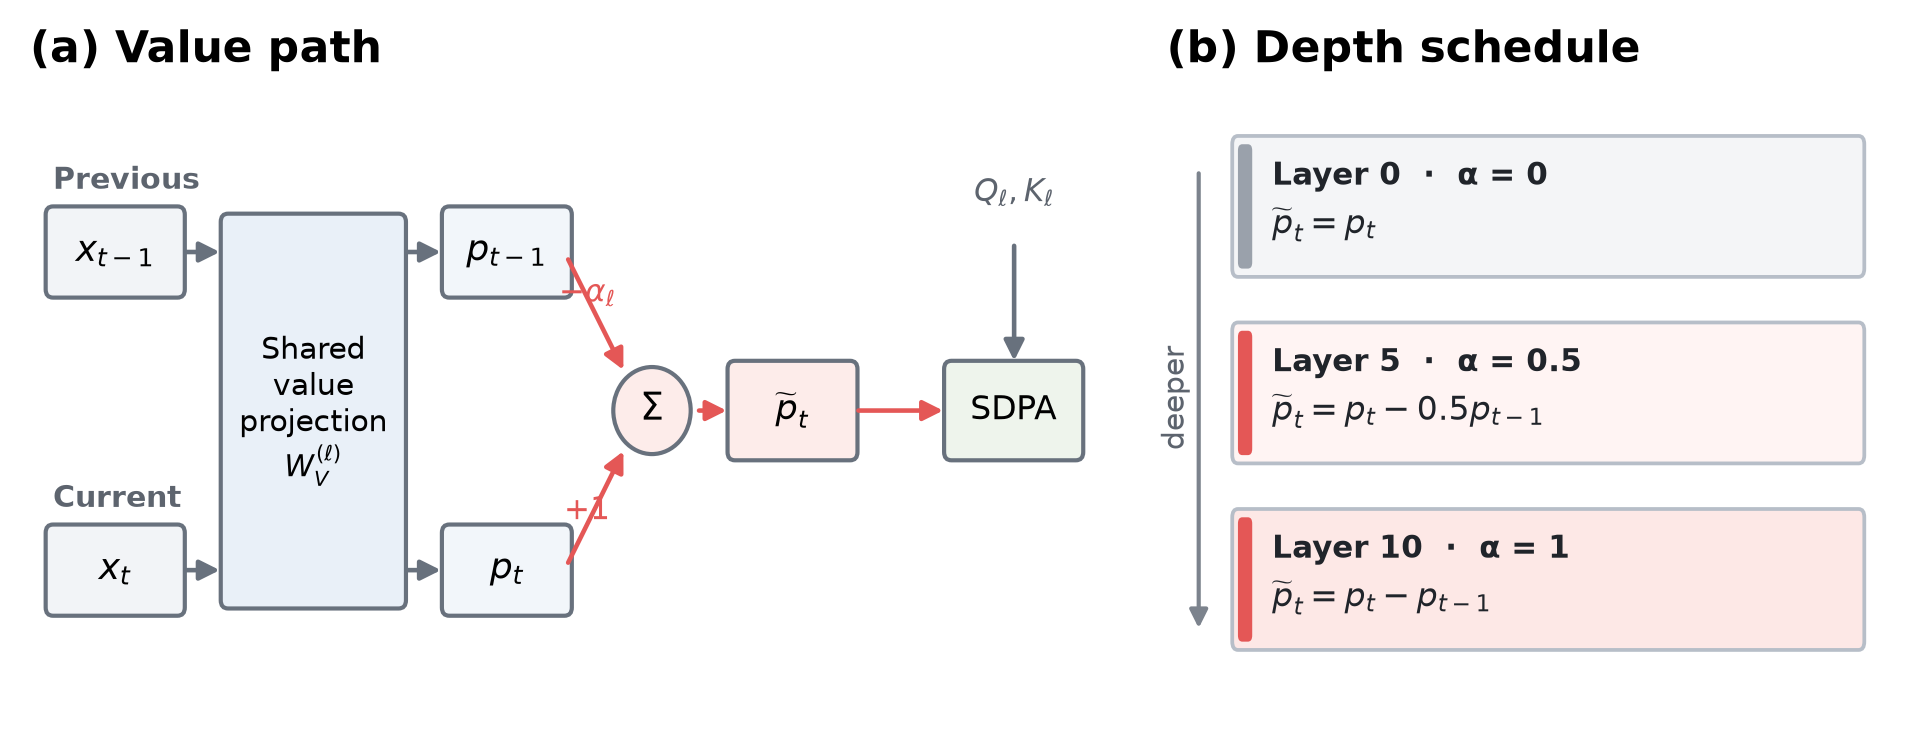
\includegraphics[keepaspectratio,alt={Value differencing changes only the payload supplied to attention. The same learned value projection processes the current and previous positions. The fixed coefficient \textbackslash alpha\_\textbackslash ell grows with depth, moving from raw values to full previous-token differences; queries and keys are unchanged.}]{figures/value_difference_mechanism.png}}
\caption{Value differencing changes only the payload supplied to attention. The same learned value projection processes the current and previous positions. The fixed coefficient \(\alpha_\ell\) grows with depth, moving from raw values to full previous-token differences; queries and keys are unchanged.}
\end{figure}

\subsection{Quantization protocol}\label{quantization-protocol}

My primary diagnostic is weights-only, per-row, round-to-nearest W4. For each eligible weight row \(w\), I compute

\[
s=\frac{\lVert w\rVert_\infty}{7}, \qquad
q=\operatorname{clip}\!\left(\operatorname{round}(w/s),-8,7\right),
\qquad \widehat w=sq.
\]

The canonical policy applies this operation symmetrically to large attention and MLP matrices in both architectures. Activations remain high precision; embeddings, normalization parameters, learned scales, and small control tensors are not quantized. I define quantization damage within each checkpoint:

\[
\Delta_{\mathrm{W4}}
=\operatorname{BPB}(\widehat\theta)-\operatorname{BPB}(\theta).
\]

Lower BPB and lower damage are better. This is intentionally a transparent diagnostic, not a substitute for GPTQ, AWQ, or a production W4A16 kernel.

\subsection{Training and evaluation}\label{training-and-evaluation}

I train matched standard and value-difference models on FineWeb with a 1,024-token vocabulary. Each model has dimension 512, 11 skip-connected blocks, eight query heads, four key/value heads, ReLU-squared MLPs, and about 27M parameters. Runs use 49 data shards, sequence length 1,024, 393,216 tokens per optimizer step, Muon for matrix parameters, and 20,000 steps. The learning rate is constant through step 17K and then decays linearly for 3K steps.

All claim-bearing endpoint and localization results use raw pre-SWA checkpoints and the same certified 256-sequence evaluator. Comparisons are paired by training seed and checkpoint. The two independent endpoint seeds are 1337 and 42; intermediate checkpoints and perturbation seeds are not counted as additional training seeds.

\subsection{Reproducibility}\label{reproducibility}

I release the evaluator, run scripts, source archives, checkpoint hashes, raw logs, machine-readable result tables, cost ledgers, preregistration snapshots, and SHA-256 manifests with the paper. The release also contains the detailed calibration, eligibility, and protocol-deviation records behind the summarized results below. Within the final control session, repeated evaluations were bit-exact; cross-session full-precision evaluation agreed within 0.000011 BPB.

\section{Quantization Reverses the Ordering}\label{quantization-reverses-the-ordering}

\subsection{Endpoints}\label{endpoints}

Figure 2 contains the central result. Standard attention is better before quantization in both seeds. After W4, value differencing is better in both. It reduces W4 damage by 18.95\% and 22.33\%, overcoming the full-precision deficit and improving post-W4 BPB by 0.00978 and 0.01782. The exact endpoint values are included in the released result table.

\begin{figure}[H]
\centering
\pandocbounded{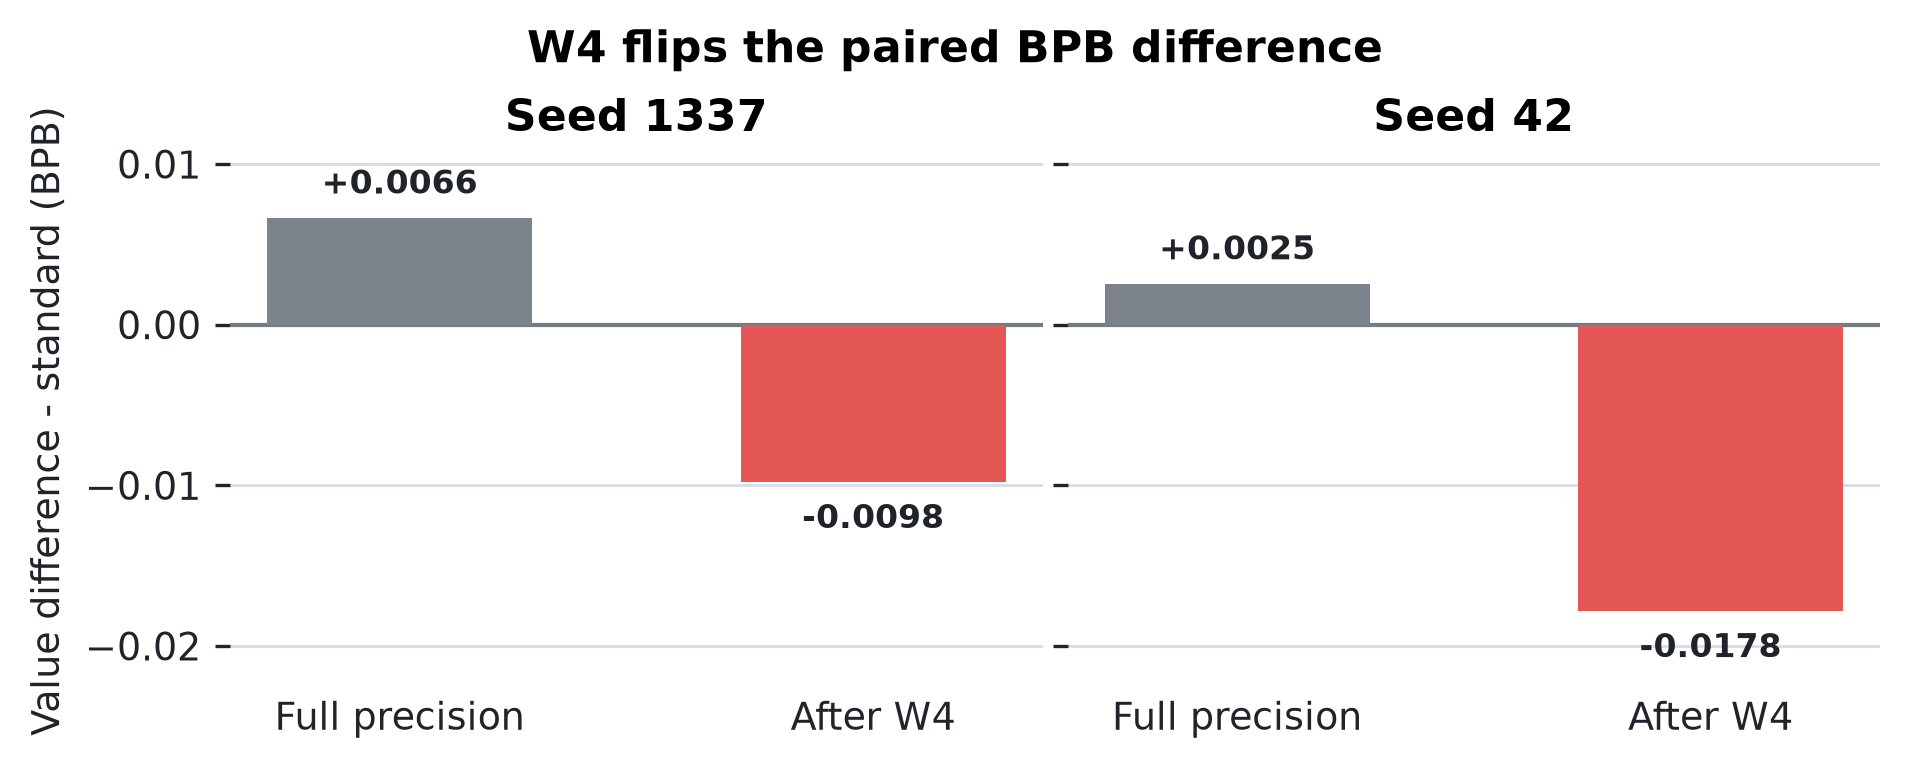
\includegraphics[keepaspectratio,alt={Paired BPB difference between value differencing and standard attention. Positive values mean standard attention has lower BPB; negative values mean value differencing has lower BPB. W4 changes the sign in both training seeds.}]{figures/int4_endpoint_reversal.png}}
\caption{Paired BPB difference between value differencing and standard attention. Positive values mean standard attention has lower BPB; negative values mean value differencing has lower BPB. W4 changes the sign in both training seeds.}
\end{figure}

The comparison is matched by training tokens, not time. Peak VRAM is tied, and the measured implementation takes 6.72\% longer per step. At four late, approximately matched-wall-clock checkpoint pairs, it wins only once. The result is therefore not compute-adjusted superiority.

\subsection{The gap persists through training}\label{the-gap-persists-through-training}

The seed-42 run saved 13 paired checkpoints from 2K to 20K steps. Value differencing takes less W4 damage at every checkpoint under the original conservative eligibility policy (Figure 3). These points are one trajectory, not 13 replications, but they show that the endpoint is not a single-checkpoint accident. The independent seed-1337 endpoint agrees in direction.

\begin{figure}[H]
\centering
\pandocbounded{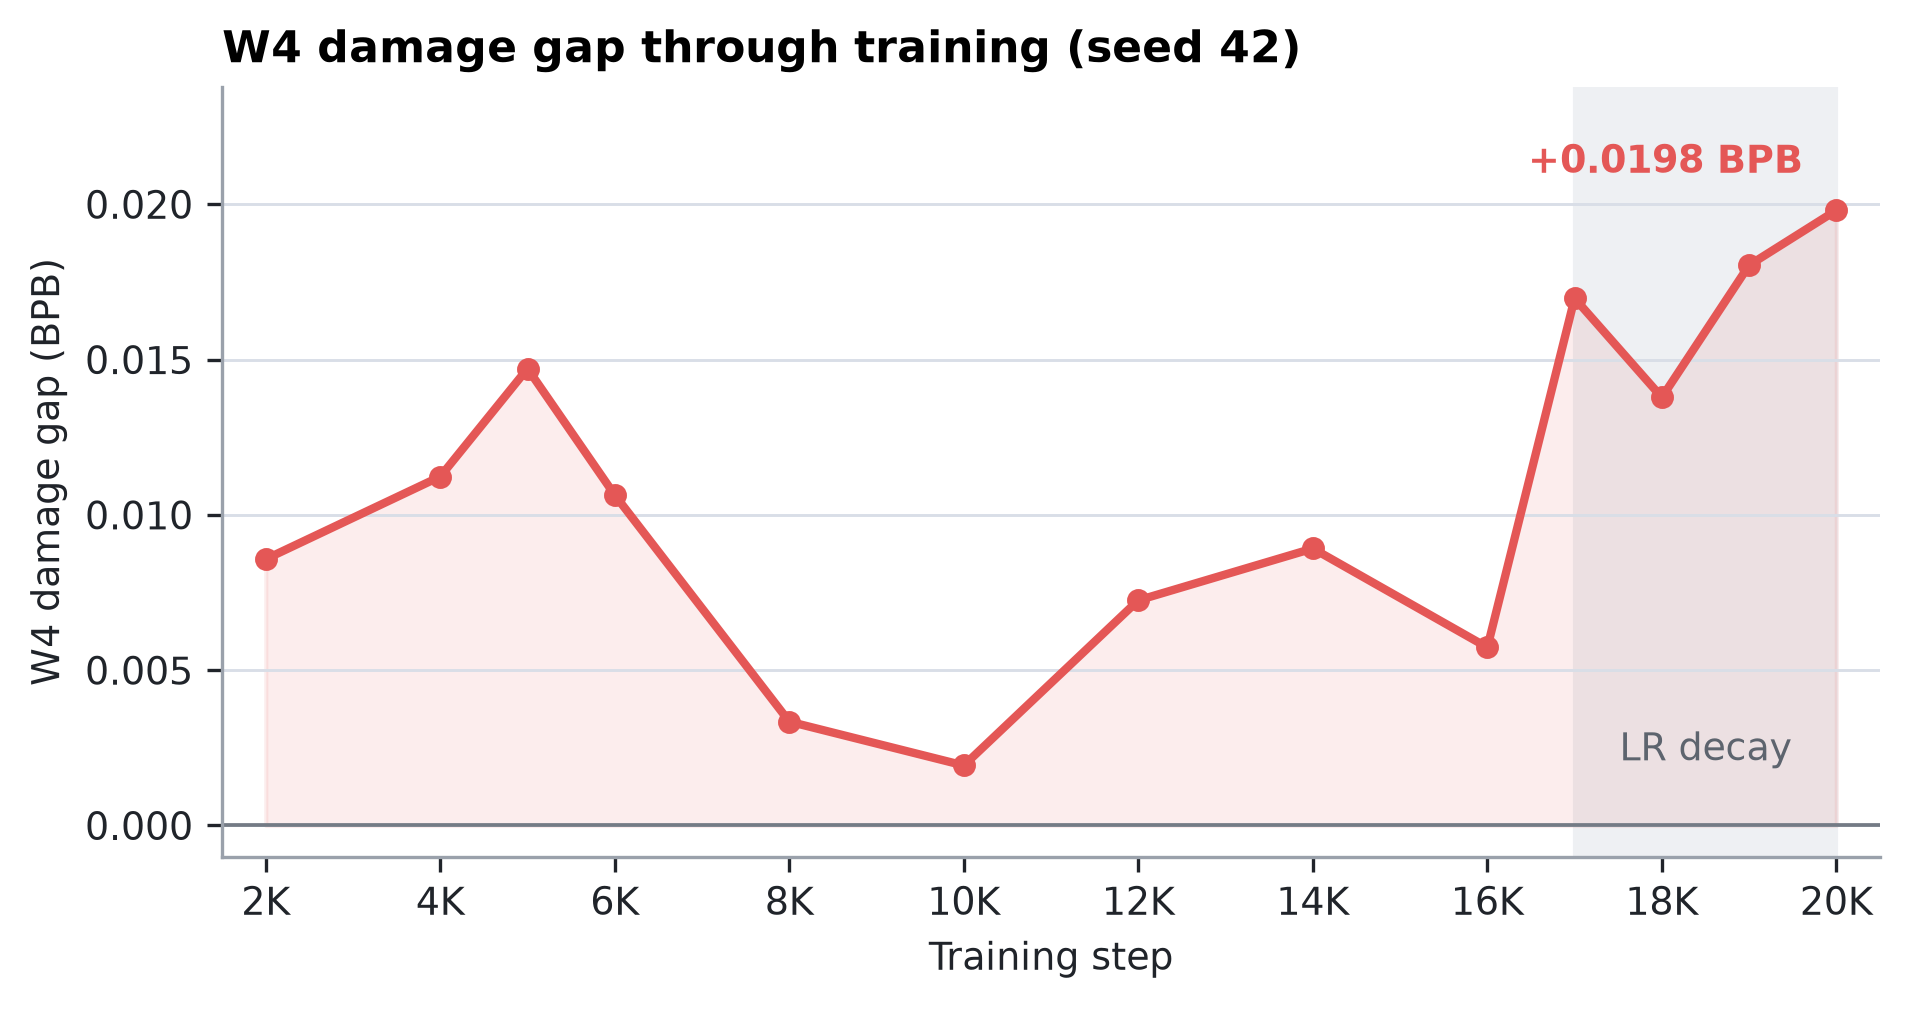
\includegraphics[keepaspectratio,alt={Standard minus value-difference W4 damage through the seed-42 run; positive values favor value differencing. The gap widens during the final learning-rate decay, from 0.00573 BPB at 16K to 0.01981 at 20K. I treat this as descriptive context, consistent with prior work on training dynamics and quantization , not as a mechanism.}]{figures/int4_damage_gap_trajectory.png}}
\caption{Standard minus value-difference W4 damage through the seed-42 run; positive values favor value differencing. The gap widens during the final learning-rate decay, from 0.00573 BPB at 16K to 0.01981 at 20K. I treat this as descriptive context, consistent with prior work on training dynamics and quantization \citep{ouyang2024undertrained,catalan2025training}, not as a mechanism.}
\end{figure}

\clearpage

\section{The Difference Lives in Attention}\label{the-difference-lives-in-attention}

\subsection{Component isolation}\label{component-isolation}

Quantizing one parameter group at a time gave a sharp answer: attention-only W4 reproduces or exceeds the entire architecture gap, whereas MLP-only W4 is null or weakly favors standard attention.

\begin{figure}[H]
\centering
\pandocbounded{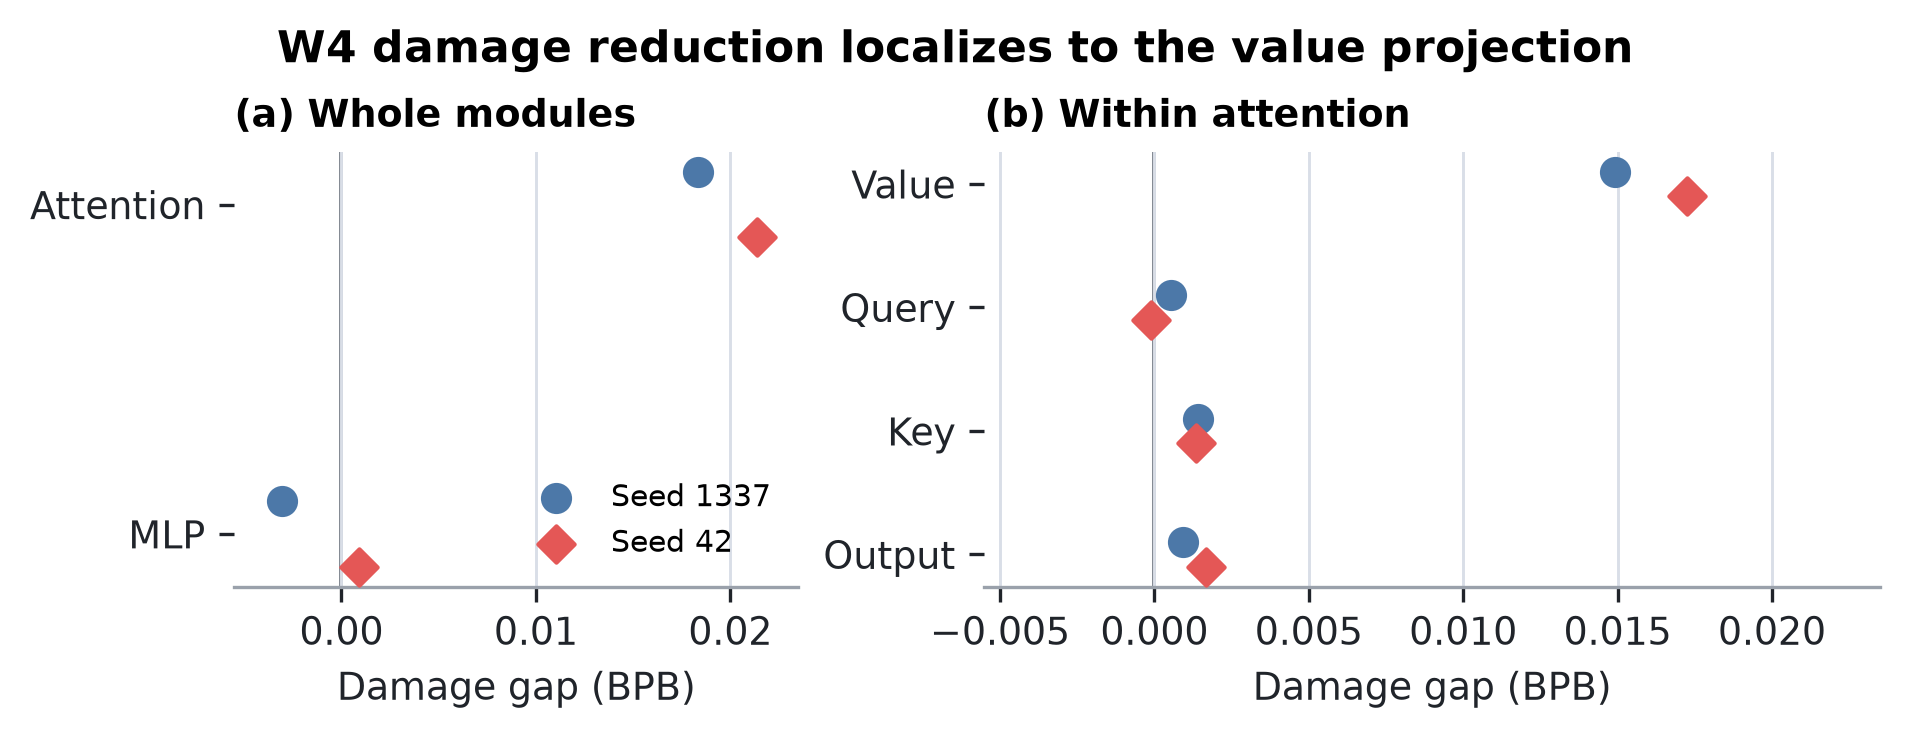
\includegraphics[keepaspectratio,alt={Standard-minus-value-difference damage by parameter group; positive values favor value differencing. The whole-module comparison is shown separately from the projections nested inside attention. Each point is a separate intervention, so the effects need not add linearly.}]{figures/int4_component_localization.png}}
\caption{Standard-minus-value-difference damage by parameter group; positive values favor value differencing. The whole-module comparison is shown separately from the projections nested inside attention. Each point is a separate intervention, so the effects need not add linearly.}
\end{figure}

The value projection alone accounts for 81.4\% and 80.7\% of the matched attention-only gap. Isolating queries, keys, or the output projection explains less than 9\% in either seed, and one query gap changes sign. The result thus localizes first to attention and then to the exact projection modified by value differencing. Exact paired damages and row provenance are included in the released component table.

This is not simply lower quantization error. Attention-weight relative RMSE is 0.11854 versus 0.11759 in seed 1337 and 0.11717 versus 0.11691 in seed 42: a 0.2--0.8\% difference in reconstruction error accompanies a 51.9--52.8\% difference in BPB damage. The same-sized numerical error has a different functional consequence.

\subsection{A perturbation control}\label{a-perturbation-control}

Round-to-nearest W4 has a particular error structure. To test whether the ordering depends on that structure, I add independent Gaussian noise to eligible attention weights at per-tensor relative RMSE 0.117. Across three paired noise seeds per training seed, every comparison favors value differencing. Mean damage falls from 0.02310 to 0.00987 BPB in seed 1337 and from 0.02266 to 0.00960 BPB in seed 42 (Figure 5).

\begin{figure}[H]
\centering
\pandocbounded{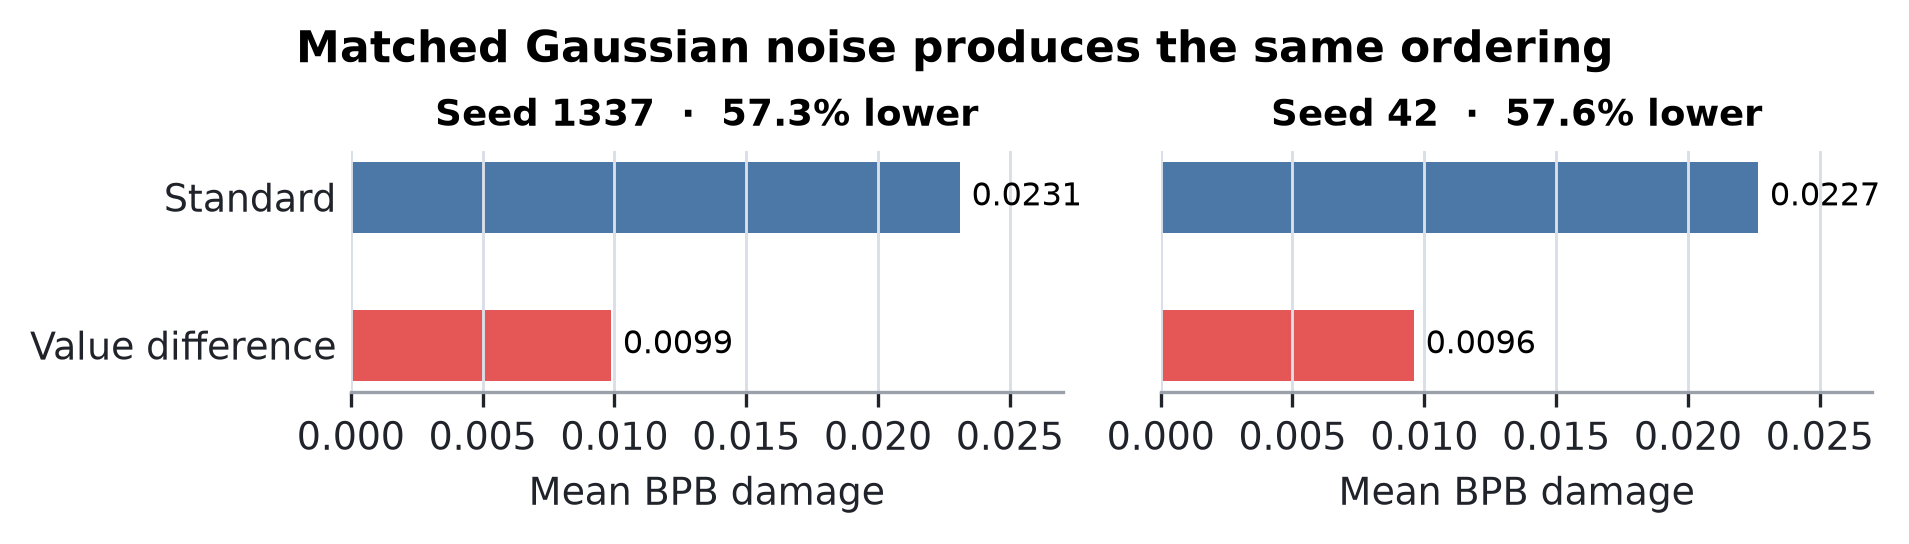
\includegraphics[keepaspectratio,alt={Mean BPB damage under RMSE-matched Gaussian perturbations of attention weights. Value differencing reduces damage by 57.3\% and 57.6\% across the two training seeds. The released control table reports all six paired noise realizations.}]{figures/gaussian_attention_control.png}}
\caption{Mean BPB damage under RMSE-matched Gaussian perturbations of attention weights. Value differencing reduces damage by 57.3\% and 57.6\% across the two training seeds. The released control table reports all six paired noise realizations.}
\end{figure}

This control rejects an explanation specific to deterministic W4 rounding. It supports lower local sensitivity within the tested attention-parameter subspace. It does \textbf{not} establish that the entire model lies in a globally flatter loss basin. The released control record documents a small historical eligibility asymmetry that biases against the modified model.

\section{What Did Not Survive}\label{what-did-not-survive}

The final claim is narrower than the project that produced it. That narrowing is evidence, not backstory to hide.

I first expected value differencing to save memory or improve full-precision quality. It did neither: tensor dimensions and peak VRAM are unchanged, and the current implementation is slower. Early pruning and dead-zone results suggested broad compression robustness, but those rankings conflicted across seeds at 20K. I then preregistered a training-maturity inversion and a cross-module compensation hypothesis; the seed-42 trajectory and branch interventions rejected both. Gentle int6 quantization is effectively a null for both models.

What survives those tests is specific and repeatable within the measured setting: W4 damage is lower, the difference is attention-local, most of it lies in the value projection, and RMSE-matched random perturbations reproduce the ordering. The released artifacts retain the complete hypothesis ledger and its dated decision rules.

\section{Interpretation}\label{interpretation}

The experiments separate \emph{error size} from \emph{error consequence}. W4 changes the two models' attention weights by nearly the same relative amount, but the change hurts standard attention roughly twice as much. Because the random-noise control agrees, the phenomenon is broader than one rounding rule. The strongest statement I can make is that value differencing lowers local sensitivity to attention-parameter perturbations in these checkpoints.

Why remains open. Value differencing may reduce the leverage of particular channels, change activation outliers, distribute payload information across neighboring positions, or guide optimization toward a less sensitive region of the attention subspace. One measured correlate points toward an outlier story: in a separate branch audit, a standard-model layer-3 MLP branch reached RMS 175.4 and maximum magnitude 134,060, versus 22.0 and 8,213 under value differencing. That measurement is not causal and did not come from the attention-W4 intervention, so I do not use it to explain the result.

\section{Related Work}\label{related-work}

Architecture-side quantizability has direct precedent. Quantizable Transformers changes attention to suppress activation outliers and enable W8A8 quantization \citep{bondarenko2023quantizable}. My result differs in both the intervention and regime: value semantics rather than softmax/no-op behavior, and weights-only W4 rather than full INT8. The shared lesson is that attention architecture can change what later compression destroys.

GPTQ and AWQ use calibration data to repair weight quantization \citep{frantar2022gptq,lin2024awq}; QuaRot and SpinQuant use rotations to reduce outliers \citep{ashkboos2024quarot,liu2024spinquant}. They are stronger deployment baselines than the transparent RTN diagnostic used here. Whether they erase or compound the architecture gap is unanswered.

KV Shifting Attention establishes learned local shifts of keys and values as prior art \citep{xu2024kvshift}. I isolate a fixed, subtractive V-side schedule and study parameter sensitivity rather than claiming token shifting itself as new. Differential Transformer is separate: it subtracts attention maps on the score side, whereas I difference value payloads across token positions \citep{ye2024differential}. Massive-activation work motivates the outlier hypothesis but does not establish it here \citep{sun2024massive}.

Finally, recent studies show that quantization behavior changes over training \citep{ouyang2024undertrained,catalan2025training}. My trajectory agrees with that broad observation. The new result is the paired architecture difference and its localization to the modified value projection.

\section{Limitations}\label{limitations}

This is a small-scale study: 27M parameters, FineWeb/SP1024, ReLU-squared MLPs, BPB evaluation, and two independent 20K training seeds. I report both seeds separately and do not claim statistical significance or a population-level effect. The quantizer is calibration-free, per-row RTN W4. I have not tested GPTQ, AWQ, production group formats, activation quantization, downstream tasks, or a real W4A16 kernel.

The implementation is 6.72\% slower per step, ties peak VRAM, and gives no consistent advantage for equal elapsed training time. Nothing here supports an inference-speed claim or production adoption. A deployment study would require larger models, modern matched-byte quantizers, downstream evaluation, and kernel-level latency and memory measurements.

The experiments establish localization and local sensitivity, not mechanism. The result may disappear with scale, a different MLP family, or a quantizer that repairs the vulnerable directions in standard attention. Those are useful boundaries for future work, not assumptions I treat as passed. Code, artifacts, and the full audit trail are available at \url{https://github.com/ddavidgao/parameter-golf}.

\section{Conclusion}\label{conclusion}

Value differencing did not deliver the full-precision win I originally sought. It did something more specific: it made the attention parameters, especially the value projection, substantially less sensitive to W4 and matched random perturbations. In two 20K seeds, that difference was large enough to reverse the post-W4 model ordering.

The practical question remains open because the experiment is small and the implementation is slower. The scientific result is nevertheless clear within its scope: changing what attention transmits can change how much damage its weights cause when perturbed, even when their numerical reconstruction error is almost the same.

\bibliography{int4_attention_refs}

\end{document}
